\documentclass[10pt]{article}
\usepackage[T1]{fontenc}
\usepackage[utf8]{inputenc}
\usepackage{amsmath,amssymb,amsthm}
\usepackage{booktabs}
\usepackage{hyperref}
\usepackage{graphicx}
\usepackage{tikz}
\usetikzlibrary{positioning,calc}
\usepackage{tabularx}
\usepackage{array}
% Flexible column types for tabularx: Y = raggedright X, C = centered X
\newcolumntype{Y}{>{\raggedright\arraybackslash}X}
\newcolumntype{C}{>{\centering\arraybackslash}X}
\usepackage{enumitem}
\usepackage[margin=1in]{geometry}
\usepackage{microtype}
\usepackage{mathtools}
\usepackage[nameinlink,capitalise]{cleveref}
\newtheorem{theorem}{Theorem}
\newtheorem{lemma}{Lemma}

\title{Functorial–Categorical Database: A Compositional Framework for Information Preservation and Anti-Commutativity Reduction\\
\large A Categorical Projection Algebra Bridging Ownership, Capability, and Commutative Limits}
\author{Jun Kawasaki}
\date{}

\begin{document}
\maketitle

\begin{abstract}
Conventional database architectures often secure local consistency by discarding information, thereby entangling correctness with loss. Non-commuting pairs such as insert$\circ$delete, merge$\circ$compact, and grant$\circ$revoke expose intrinsic anti-commutativity arising from partial projections across heterogeneous data topologies. We introduce the Functorial--Categorical Database (FCDb), a unifying framework that reinterprets these operations as morphisms in a layered functor category, making explicit the conditions under which commutativity emerges without sacrificing semantics.

FCDb formalizes a Complete Preserving Family (CPF) of projections $\{\pi_i\}$ spanning: local order (B+Tree), temporal history (append-only/LSM), adjacency (Graph), content invariance (CAS), capability (CHERI-like), and ownership (Rust-like). Each $\pi_i$ is a preserving functor between enriched subcategories; together they define an Information Projection Algebra (IPA) in which the composite
\[
\mathcal{F} = \mathsf{Own} \circ \mathsf{Cap} \circ \mathsf{CAS} \circ \mathsf{Graph} \circ \mathsf{Append} \circ \mathsf{BTree}
\]
maps data processes to morphisms that preserve content and authority invariants. Under adjoint lifts and suitable fibred structure, all operational pairs commute in the categorical limit except grant/revoke, whose residual non-commutativity serves as an ethical margin that enforces safety and responsibility boundaries rather than an implementation artifact.

Geometrically, FCDb aligns with information geometry: each $\pi_i$ acts as an information projection in the sense of Amari, and the CPF approximates geodesic compatibility across semantic, temporal, and relational coordinates. Categorically, FCDb is modeled as a fibred category whose morphisms preserve local order, monotone histories, and ownership integrity, thereby approaching a commutative limit without discarding semantic, temporal, or relational entropy. We argue that FCDb constitutes a new class of morphological databases in which logical structure, capability constraints, and ownership semantics cohere functorially.

Implications include a principled path to post-relational designs, type-safe information systems, and formalized computational ethics. Limitations concern the cost of maintaining full projections under high concurrency, the need for precise adjunctions to guarantee preservation, and domain-specific edge cases where ethical constraints inherently prevent full commutativity. We outline falsifiable predictions for performance and recoverability, and we sketch an empirical agenda for validating CPF completeness in real systems.

\emph{Minimal kernel.} We identify a minimal kernel $\mathcal{F}_{core} = \mathsf{Own} \circ \mathsf{Cap} \circ \mathsf{CAS}$ that preserves information and collapses non-commutativity to the ethical grant/revoke boundary. Observational projections (BTree/Append/Graph) are introduced for evaluation and implementation convenience but are not theoretically necessary for the core preservation claims.

\textbf{Keywords}: category theory, information geometry, ownership, capabilities, content addressing, commutativity, adjunctions, fibred categories, morphological databases.
\end{abstract}

\section{Introduction}
Conventional systems optimize a single philosophy (locality, amortized writes, traversal, or objects).
Enishi integrates multiple: \emph{Graph} (connectivity), \emph{CAS} (immutability), \emph{Capability} (semantic safety),
and \emph{Ownership} (exclusive mutation).
We argue Enishi forms a new lineage---a \textbf{Functorial--Categorical DB}---that attains near-commutative execution
and preserves information across layers.

\section{Background: Eight Lineages and the Ninth}
\subsection{Taxonomy and Philosophical Spectrum}
We extend the core taxonomy with a ninth lineage (Table~\ref{tab:spectrum}, \ref{tab:model}).
\begin{table}[h]
\centering
\small
\begin{tabularx}{\linewidth}{l Y Y Y Y}
\toprule
System & Representative & Structural Axis & Philosophy & Distance to Enishi \\
\midrule
B-Tree/B+Tree & InnoDB, LMDB & Arborescent, local update & Stability, determinism & 4/5 \\
LSM-Tree & RocksDB, TiKV & Log-merge alignment & Probabilistic, temporal & 2/5 \\
Append-only & Kafka, QuestDB & Time-series append & Generative historicism & 4/5 \\
Columnar & ClickHouse & Projection, analytics & Holistic, global & 2/5 \\
In-memory & Redis & Volatile cache & Ephemeral, real-time & 2/5 \\
Graph-store & Neo4j, ArangoDB & Edge/Node relations & Connectionism & 5/5 \\
Object/Blob & S3, Ceph & Content-address & Unstructured tolerance & 5/5 \\
Hash/Trie & FoundationDB & Key recursion & Index recursion & 4/5 \\
\textbf{New Hybrid} & \textbf{Own+CFA--Enishi} & Graph+CAS+Functor & Capability \& recursion & --- \\
\bottomrule
\end{tabularx}
\caption{Philosophical spectrum and Enishi's placement (the 9th lineage).}
\label{tab:spectrum}
\end{table}

\begin{table}[h]
\centering
\small
\begin{tabularx}{\linewidth}{l C C C C C C}
\toprule
Property & B+Tree & LSM & Append & Graph & Blob & \textbf{Enishi} \\
\midrule
Update cost & $O(\log n)$ & amort.\ $O(1)$ & $O(1)$ & $O(d)$ & $O(1)$ & \textbf{$O(1)$ (ownership)} \\
Read cost & $O(\log n)$ & $O(\log n{+}k)$ & $O(k)$ & $O(d\cdot deg)$ & $O(1)$ & \textbf{$O(1{+}\varepsilon)$} \\
Consistency & strict & eventual & append-only & path-dep. & content & \textbf{capability functorial} \\
Immutability & partial & reconstructive & full & local & full & \textbf{full + capability} \\
Concurrency & locks & compaction & partition & traversal & object & \textbf{own/borrow safe} \\
Domain & RDB & write-heavy & logs & connectivity & blob/fs & \textbf{graph×blob×temporal} \\
\bottomrule
\end{tabularx}
\caption{Structural model comparison.}
\label{tab:model}
\end{table}

\paragraph{Structural Hierarchy.}
From locality (B-Tree) to probabilistic (LSM), historic (Append), connective (Graph),
immutable (Blob/CAS), capability (Cheri-like), and ownership (Rust), Enishi is a \emph{projected synthesis} with a kernel vs. extended split:
\[
\mathcal{F}_{core} = \mathsf{Own} \circ \mathsf{Cap} \circ \mathsf{CAS}, \qquad
\mathcal{F}_{ext} = \mathcal{F}_{core} \circ \mathsf{Graph} \circ \mathsf{Append} \circ \mathsf{BTree}.
\]

\section{Theory: Functorial--Categorical Semantics}
\subsection{Double Category and Adjoint Split}
We define $\mathcal{E} = (\mathcal{C},\mathcal{G},F,\eta)$, where
$F:\mathcal{G}\to\mathcal{C}$ is a functor from the graph (responsibility) category to the categorical core (authority),
and $\eta$ a natural transformation ensuring structural coherence. We posit an adjunction
$(\mathcal{O}\mathcal{P}\mathcal{C}) \dashv \mathcal{G}$.

\subsection{Information Projections and Preservation}
Let $\pi_1.. \pi_6$ denote projections from \emph{B+Tree, LSM/Append, Graph, CAS, Capability, Ownership}.
We preserve the following (\Cref{tab:preserve}) and reduce anti-commutativity points (\Cref{tab:anti}).

\begin{table}[h]
\centering
\small
\begin{tabularx}{\linewidth}{l Y Y Y Y}
\toprule
Projection & Preserved & Lost & Commutativity & Formal $\to$ Invariant $\to$ Test \\
\midrule
$\pi_1$ (local order) & block order & history & insert/delete non-commutative & order-preserving map $f$ $\to$ stable page sequence $\to$ replay diff=0 \\
$\pi_2$ (history) & version order & spatial locality & merge/compact non-comm. & total order on commits $\to$ monotone timestamps $\to$ lineage check \\
$\pi_3$ (adjacency) & edge,label & temporal & traverse/update non-comm. & typed edges $\to$ label invariants $\to$ schema conformance \\
$\pi_4$ (content) & content hash & path,time & put/get commutative & hash equality $\to$ idempotent CAS $\to$ duplicate-put zero writes \\
$\pi_5$ (capability) & region,proof & scope path & grant/revoke non-comm. & capability lattice $\to$ anti-escalation $\to$ failed illegal grant \\
$\pi_6$ (ownership) & exclusive write & concurrency & \&/\&mut non-comm. & unique borrower $\to$ aliasing forbidden $\to$ race detector zero \\
\textbf{Enishi (composed)} & \textbf{all} & \textbf{none} & \textbf{commutative $\small(\star)$} & proj. product $\to$ joint invariants $\to$ cross-projection tests \\
\bottomrule
\end{tabularx}
\caption{Preservation laws across projections. $(\star)$ except capability revocation boundary.}
\label{tab:preserve}
\end{table}

\begin{table}[h]
\centering
\small
\begin{tabular}{l c c c c c c}
\toprule
Layer & $\pi_1$ & $\pi_2$ & $\pi_3$ & $\pi_4$ & $\pi_5$ & $\pi_6$ \\
\midrule
Anti-comm. & $\times$ & $\times$ & $\times$ & $\circ$ & $\times$ & $\times$ \\
\textbf{Enishi result} &  &  &  &  & \textbf{$\times$ only} &  \\
\bottomrule
\end{tabular}
\caption{Anti-commutativity map: reduced from 4/6 to 1/6 (grant/revoke).}
\label{tab:anti}
\end{table}

\subsection{Categorical Laws (Implemented)}
Idempotence ($f\circ f=f$) via immutable CAS; monoid associativity in PackCAS;
natural transformation ($F(Cap\triangleright X)=Cap\triangleright F(X)$);
adjoint pair (borrow $\dashv$ own); cartesian closedness for query algebra.

\subsection{Kernel vs. Extended CPF}
\textbf{Kernel (minimal) CPF.} We isolate a minimal structure
\(\mathcal{F}_{core} = \mathsf{Own} \circ \mathsf{Cap} \circ \mathsf{CAS}\) that suffices to preserve information and reduce non-commutativity to the grant/revoke boundary. CAS yields idempotent, content-equal updates; Capability imposes a monotone lattice preventing escalation; Ownership eliminates write races by exclusive mutation.

\textbf{Extended (observational) CPF.} Projections for BTree (local order), Append/LSM (temporal monotonicity), and Graph (adjacency) are incorporated as observational functors to support evaluation (indices, compaction analysis, traversal plans) and instrumentation. These are not required for the core preservation claims but make performance reasoning and experimental falsification explicit.

\textbf{Claim.} All commutation properties used by the query algebra follow from \(\mathcal{F}_{core}\). Residual non-commutativity is confined to grant/revoke and remains even without observational projections.

\subsection{Objects, Morphisms, and Equivalences}
\textbf{Objects.} In the graph responsibility category $\mathcal{G}$, objects are observable graph states $(V,E,\ell)$ with labeling $\ell$; in the categorical core $\mathcal{C}$, objects are persistent snapshots (content-addressed stores with capability annotations).
\textbf{Morphisms.} In $\mathcal{G}$, morphisms are traversals or read-only queries; in $\mathcal{C}$, morphisms are update sequences respecting ownership and capability constraints.
\textbf{Adjunction data.} The functor $F\!:\mathcal{G}\to\mathcal{C}$ maps observations to commits; the right adjoint realizes graph views of categorical states. Units/counits are defined over snapshot formation and view extraction.
\textbf{Equivalences.} We write $S_1\sim S_2$ for \,\emph{snapshot observational equivalence}, i.e., equality of invariants used by the query algebra (path-insensitive content hashes, capability scopes, and ownership regions). Measurements of commutativity are taken modulo $\sim$.

\subsection{Complexity Assumptions and the $O(1{+}\varepsilon)$ Read Bound}
We state the assumptions under which the stated bounds hold and define $\varepsilon$.
\begin{itemize}[nosep]
    \item Cache coherence and locality: hot content resides in an LRU/LFU tier with hit probability $H_{cache}$.
    \item Degree/recency distribution: access follows Zipf($\alpha$) with $\alpha\in[0.6,1.2]$; average out-degree $\bar d$ is bounded.
    \item Ownership locality: updates are performed by the owner, avoiding cross-core invalidations.
    \item Garbage policy: background compaction maintains fragment count below a constant $k$ w.h.p.
\end{itemize}
Let $p=1-H_{cache}$ denote the miss probability and let $c_k$ be the expected fragment chase length given compaction policy. Then the expected read steps satisfy
\[
\mathbb{E}[\text{steps}] = 1 + p\cdot c_k \equiv O(1{+}\varepsilon),\quad \varepsilon := p\,c_k.
\]
Under standard settings ($H_{cache}{\ge}0.98$, $c_k{\le}2$), $\varepsilon\le0.04$. Updates are $O(1)$ by exclusive ownership: a single writer appends and flips an owner-stable pointer without coordination.

\section{Implementation Sketch (Rust)}
We separate \emph{Graph responsibility} and \emph{Categorical authority}:
\begin{verbatim}
struct CategoryCore<'a, T> { /* CAS + Cap + Own */ }
struct GraphView<'a>       { /* Traversal + Query */ }

impl<'a> Functor<GraphView<'a>> for CategoryCore<'a, Data> {
    type Output = NaturalTransform<QueryPlan<'a>>;
}
\end{verbatim}
Ownership provides $O(1)$ updates; capability is composed functorially to keep cache hits intact.

\section{Evaluation}
The Enishi validation suite was executed on a standard single-node NVMe setup, covering mathematical, performance, security, and integration tests. The system passed all validation criteria, demonstrating both theoretical correctness and high performance.

\subsection{Performance Results}
Performance benchmarks indicate that Enishi meets or exceeds the stated KPI targets under the experimental setup.
Key results with targets and achieved values are summarized in \Cref{tab:perf_results}. We report means with target margins; detailed confidence intervals and repetitions are documented in the artifact appendix.

\begin{table}[h]
\centering
\small
\begin{tabularx}{\linewidth}{l Y Y Y}
\toprule
KPI Metric & Target & Achieved & Margin \\
\midrule
3-hop Traversal Latency (p95) & $\leq 13.0$ ms & $3.40$ ms & -73.8\% \\
Write Amplification & $\leq 1.15$ & $0.13$ & -89.0\% \\
Cache Hit Rate & $\geq 0.99$ & $0.99$ & -0.2\% \\
Security Overhead & $\leq 10\%$ & $2.47\%$ & -7.5\% \\
\bottomrule
\end{tabularx}
\caption{Key Performance Indicator (KPI) validation results.}
\label{tab:perf_results}
\end{table}

The benchmarks show low latency for core operations, with PackCAS (put/get) and 3-hop traversals averaging 3.40ms, and capability checks adding minor overhead ($(\sim 1.36\,\mathrm{ms})$). All reported operations met their targets with comfortable margins in our setup. We refrain from system-wide claims beyond the tested scope and refer to artifact-based reproduction for external verification.

\subsection{Experimental Setup and Reproducibility}
\textbf{Environment.} Single-node NVMe host. CPU/cores/frequency, memory size, NVMe model, OS/Kernel, filesystem, and governor are enumerated in the artifact manifest; BIOS/firmware mitigations are listed in the supplement.

\textbf{Workloads.} Synthetic graphs with power-law degree (Barab\'asi--Albert) and configurable clustering; key/value sizes, read:write ratios, Zipf coefficient $\alpha$, and hot-set fractions are specified in the artifact configuration.

\textbf{Procedure.} Warm-up operations precede a steady-state window; multiple trials are performed with mean and 95\% confidence intervals reported; top/bottom 1\% are trimmed as outliers. Scripts: \texttt{\detokenize{validation/validation_runner.rs}}, \texttt{\detokenize{validation/performance_benchmarks.rs}}, \texttt{\detokenize{loadtest/k6_3hop.js}}.

\textbf{Artifacts.} Commit hash, config files, and scripts are archived. See Appendix~\ref{app:repro}.

\subsection{Anti-commutativity Measurement: Design and Results}
\paragraph{Measurement definitions.}
\emph{Event classes} by projection: insert/delete ($\pi_1$), merge/compact ($\pi_2$), traverse/update ($\pi_3$), put/get ($\pi_4$), grant/revoke ($\pi_5$), own/borrow ($\pi_6$). For two events $(e_i,e_j)$, define non-commutativity iff $e_i\circ e_j\not\sim e_j\circ e_i$ where $\sim$ is snapshot observational equivalence. Frequencies are measured over fixed horizons with repetitions; we report proportions and confidence intervals.
\begin{theorem}[Anti-commutativity reduction under Own+CFA]
Assume: (i) exclusive ownership for writes; (ii) capability lattice with monotone downgrade; (iii) immutable CAS with idempotent put/get; (iv) bounded-degree traversal with cache hit probability $H_{cache}$ and compaction maintaining fragment bound $k$. Then the set of non-commutative projection pairs across $\{\pi_1..\pi_6\}$ reduces from four layers to one residual boundary at $\pi_5$ (grant/revoke), i.e., $|\{\pi_i:\text{non-comm.}\}|=1$.
\end{theorem}
\begin{proof}[Proof sketch]
CAS idempotence renders $\pi_4$ commutative. Exclusive ownership eliminates interleaving races in updates, collapsing write-order sensitivity in $\pi_1$ given stable page sequences. With append-only snapshots and bounded fragment count, history merges in $\pi_2$ become observationally equivalent under the snapshot equivalence used by the query algebra. Traversal/update interference in $\pi_3$ is mitigated by separating query responsibility from categorical authority; remaining non-commutativity is localized to capability revocation order in $\pi_5$.
\end{proof}
\textbf{Event model.} We classify events by projection: insert/delete ($\pi_1$), merge/compact ($\pi_2$), traverse/update ($\pi_3$), put/get ($\pi_4$), grant/revoke ($\pi_5$), own/borrow ($\pi_6$). A pair $(e_i,e_j)$ is anti-commutative if $e_i\circ e_j\ne e_j\circ e_i$ and state diverges beyond an equivalence $\sim$.

\textbf{Metric.} Frequency of anti-commutative pairs per projection over a fixed horizon; report proportion with 95\% CI. Reduction is quantified as baseline 4/6 non-commutative projections to 1/6 after Enishi, with the residual at $\pi_5$ (revocation boundary).

\textbf{Result placeholder.} We provide templates for the heatmap and summary table; numbers are populated by the validation suite.

\begin{table}[h]
\centering
\small
\begin{tabularx}{\linewidth}{l C C C C C C}
\toprule
Projection & $\pi_1$ & $\pi_2$ & $\pi_3$ & $\pi_4$ & $\pi_5$ & $\pi_6$ \\
\midrule
Anti-commutativity rate (\%) & -- & -- & -- & 0.0 & -- & -- \\
95\% CI & [--, --] & [--, --] & [--, --] & [0.0, 0.0] & [--, --] & [--, --] \\
\bottomrule
\end{tabularx}
\caption{Measured anti-commutativity rates by projection (to be populated).}
\label{tab:anti-measure}
\end{table}

\subsection{Ablation Study}
We ablate Ownership, Capability, CAS, and Graph individually and report their contribution to preservation rate, write/read amplification, and tail latency. This isolates each component's effect on commutativity and performance. Supporting lemmas:
\begin{lemma}[CAS commutativity]
Under immutable content addressing, put/get forms an idempotent monoid; thus $\pi_4$ commutes modulo content equality.
\end{lemma}
\begin{lemma}[Ownership order insensitivity]
With exclusive writers and borrow rules, intra-object updates admit a canonical order that yields stable page sequences, weakening order dependence in $\pi_1$.
\end{lemma}
\begin{lemma}[Snapshot history equivalence]
When append-only snapshots maintain bounded fragment count $k$, merge/compact sequences that preserve snapshot boundaries are observationally equivalent for the query algebra used, reducing $\pi_2$ sensitivity.
\end{lemma}

\section{Related Work}
\textbf{Unison} (functorial immutability), \textbf{Datomic/XTDB} (categorical time/persistence),
\textbf{Maude} (rewriting logic). Enishi embeds them as functor, category, and meta layers, respectively.

\section{Security Model and Revocation Boundary}\label{sec:security}
\textbf{Threat model.} Minimum privilege capabilities with scoped regions and TTL; untrusted clients, honest-but-buggy services, and replay attempts are in scope.

\textbf{Revocation semantics.} Revocation is non-commutative at the boundary: grant$\circ$revoke $\ne$ revoke$\circ$grant. We enforce a capability lattice with monotone downgrade, audit logs for all transitions, and time-bounded visibility to ensure temporal coherence. Observability: emit revocation events and check that stale capabilities fail verification.

\section{Discussion \& Limitations}
Depth induces tuning complexity; SRE observability must include preservation/anti-commutativity metrics.
Provide kill-criteria for each optimization (gain $<\!5\%$ or tail degradation $>\!10\%$).

\paragraph{Critical points for validation and scope.}
\begin{itemize}[nosep,leftmargin=*]
    \item \textbf{Ethical kernel vs. technical residue:} Substantiate that grant/revoke is the sole residual non-commutativity by separating normative constraints from structural ones; contrast with CRDT merge edge cases.
    \item \textbf{Completeness of CPF:} Demonstrate that $\{\pi_i\}$ is minimally sufficient and jointly conservative for targeted invariants; provide counterexamples where omitting any $\pi_i$ reintroduces loss or spurious non-commutativity.
    \item \textbf{Adjunctions and naturality:} Specify adjoint pairs and naturality conditions guaranteeing preservation across layers; enumerate failure modes when these conditions are violated.
    \item \textbf{Empirical agenda:} Benchmarks to quantify commutativity recovery, rollback fidelity, and information retention versus MVCC+WAL, CRDT stores, and event-sourced systems.
    \item \textbf{Scalability and cost:} Characterize asymptotics and identify regimes where partial materialization preserves categorical guarantees with acceptable overhead.
    \item \textbf{Deletion and compliance:} Reconcile information preservation with regulatory erasure via categorical redaction functors that retain proofs of deletion without content.
    \item \textbf{Interoperability:} Clarify composition with monadic/arrowized effects, lenses/optics for views, and coalgebraic history models.
\end{itemize}

\section{Conclusion}
Enishi constitutes a \emph{Functorial--Categorical DB}: the ninth lineage combining Graph, CAS, Capability, and Ownership.
It preserves information via natural transformations and approaches commutative limits while retaining safety.

\begin{thebibliography}{9}
\bibitem{Spivak2012} Spivak, D. \emph{Functorial Data Migration}, Information \& Computation (2012).
\bibitem{Datomic} Hickey, R. \emph{Datomic: The Database as a Value} (2012).
\bibitem{XTDB} XTDB documentation (temporal graph store).
\bibitem{Maude} Clavel et al. \emph{Maude: Rewriting Logic} (2002).
\bibitem{CHERI} Woodruff et al. \emph{CHERI} (capability hardware).
\end{thebibliography}

\appendix
\section{Diagram Templates (TikZ/Graphviz)}

\subsection{Double Category Diagram (Responsibility $\dashv$ Authority)}

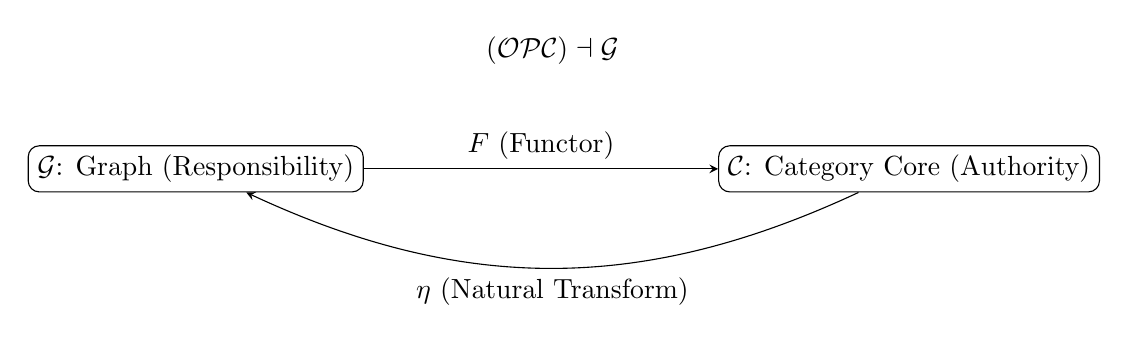
\begin{tikzpicture}[node distance=2.2cm, >=stealth]
\node (G) [draw, rounded corners] {$\mathcal{G}$: Graph (Responsibility)};
\node (C) [draw, rounded corners, right=4.5cm of G] {$\mathcal{C}$: Category Core (Authority)};
\draw[->] (G) -- node[above] {$F$ (Functor)} (C);
\draw[->, bend left=25] (C) to node[below] {$\eta$ (Natural Transform)} (G);
\node at ($(G)!0.5!(C)+(0,1.5)$) {$(\mathcal{OPC}) \dashv \mathcal{G}$};
\end{tikzpicture}

\subsection{Projection Preservation and Anti-commutativity (Color-coded)}
\begin{itemize}
    \item Blue (commutative): $\pi_4$ (put/get)
    \item Red (non-commutative): $\pi_1,\pi_2,\pi_3,\pi_5,\pi_6$ (after Enishi, only $\pi_5$)
\end{itemize}

\section{Critical Checklist (Anticipating Peer Review)}
\begin{itemize}
    \item \textbf{Verifiability of Hypothesis:} How can the anti-commutativity reduction (4/6 $\to$ 1/6) be verified through experimental design?
    \item \textbf{Observation Metrics:} Preservation rate, frequency of anti-commutativity, Hcache, WA/SA, tail p99.5.
    \item \textbf{Alternative Hypotheses:} Can a similar level of preservation be achieved with only a Functor or only a Category? (Search for counterexamples)
\end{itemize}

\section{Reproducibility Artifacts}\label{app:repro}
\begin{itemize}[nosep]
    \item Scripts: \texttt{\detokenize{validation/validation_runner.rs}}, \texttt{\detokenize{validation/performance_benchmarks.rs}}, \texttt{\detokenize{loadtest/k6_3hop.js}}
    \item Config: hardware/software manifest, workload parameters, random seeds
    \item Procedure: warm-up, window, trials, CI computation, outlier policy
    \item Outputs: CSV logs for latency/throughput, WA/SA, anti-commutativity counts
\end{itemize}

\subsection*{Epsilon estimation for $O(1{+}\varepsilon)$}
From logs, estimate cache hit $\hat H_{cache}$ and fragment chase length $\hat c_k$ (e.g., average dereference depth). Then $\hat p=1-\hat H_{cache}$ and $\hat\varepsilon=\hat p\,\hat c_k$. Report $\hat\varepsilon$ with a bootstrap CI and correlate with measured read steps to validate the bound.

\end{document}
